\input{header}

\AtBeginSubsection[]
{
	\begin{frame}<beamer>
		\frametitle{Outline}
		\tableofcontents[current,currentsubsection]
	\end{frame}
}

\begin{document}

\begin{frame}[allowframebreaks,containsverbatim] \frametitle{Nondeterministic TM $
\equiv$ deterministic TM}
  \begin{itemize}
\item A language recognized by TM
$\Rightarrow$ recognized by NTM
\item
  [] A deterministic TM is a nondeterministic TM
\item A language recognized by NTM
$\Rightarrow$ recognized by TM
\item
  [] more difficult
\item
  We must simulate NTM by TM
\item
  How did we run NTM?
\item[]
  Like NFA we use a tree for processing the input
(\# branches finite)
\item
  To traverse a tree we can do
  \begin{center}
  depth-first search
\end{center}
  or
  \begin{center}
  breadth-first
\end{center}
\item If using depth-first search, one branch 
may lead to $\infty$ steps
\item [] Then we cannot consider other branches even if the
  input is accepted

  
\item
  Thus we should consider breadth-first
  
\item Fig 3.17: a deterministic TM to simulate a nondeterministic TM

\begin{center}
  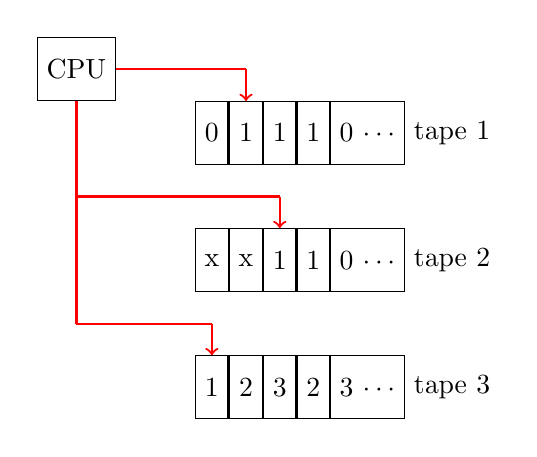
\begin{tikzpicture}[ampersand replacement=\&]
\matrix[nodes={minimum height=8mm}]     
{
  \node[draw](0) {CPU}; \& [1cm]  \& \node(1){} ; \&\&\& \& \\
  \& \node[draw]{0}; \& \node[draw](a){1}; \& \node[draw]{1}; \& \node[draw]{1};  \& \node[draw]{0 $\cdots$};  \& \node{tape 1};\\
\node(2){} ; \&  \&  \& \node(21){} ; \&\& \&\\  
\& \node[draw]{x}; \& \node[draw]{x}; \& \node[draw](b){1}; \& \node[draw]{1}; \& \node[draw]{0 $\cdots$}; \& \node{tape 2};  \\
\node(3){} ; \& \node(31){} ; \&  \&\& \& \&\\
\& \node[draw](c){1}; \& \node[draw]{2}; \& \node[draw]{3}; \& \node[draw]{2}; \& \node[draw]{3 $\cdots$}; \&  \node{tape 3}; \\
};

\draw [-,red,thick] (0) -- (1.center) ;
\draw [->,red,thick] (1.center) -- (a) ;
\draw [-,red,thick] (0) -- (2.center) ;
\draw [-,red,thick] (2.center) -- (21.center) ;
\draw [->,red,thick] (21.center) -- (b) ;
\draw [-,red,thick] (0) -- (3.center) ;
\draw [-,red,thick] (3.center) -- (31.center) ;
\draw [->,red,thick] (31.center) -- (c) ;
\end{tikzpicture}
\end{center}
  
\item 
Tape 1: input, never altered

\item
  Tape 2: copy input from tape 1 and run one branch up to certain layer
  
\item
  Tape 3: store a path to a node

\item
  The key is the 3rd tape

\item
  Suppose $\max$ \# branches 3

\item If contents of 3rd tape are
  \begin{center}
    231
  \end{center}
  it means
  \begin{center}
      root $\rightarrow$ 2nd child $\rightarrow$ 3rd child $\rightarrow$ 1st child
  \end{center}
\item Thus tape 3 contents in the procedure can be like
\begin{alltt}
1
2
3
11
...
33
111
...
333
\end{alltt}
\item What if say 111 is not a valid configuration? For example,
  after 11, there is no link to go to the 1st child
\item That is fine. We can still check such a path as long as it
  is finite
\item Therefore, an NTM can be simulated by a three-tape TM
\item
  We have shown that a multi-tape TM can be simulated
  by a single-tape TM
\item
  Thus the proof is completed
\end{itemize}\end{frame}

% \begin{frame}[allowframebreaks] \frametitle{Corollary 3.18}
%   \begin{itemize}
% \item omit

% \end{itemize}\end{frame}

\begin{frame}[allowframebreaks] \frametitle{Corollary 3.19}
  \begin{itemize}
\item Definition: NTM is a decider if all branches halt on all inputs


\item Language decidable $\Leftrightarrow$
some NTM decides it

\item
  $\Rightarrow$ easy, one TM decides it and a TM is an NTM

\item
  [] This TM halts on all inputs (one branch)

\item
  $\Leftarrow$:
\item
  [] Now NTM terminates on all branches 

\item
  [] We can construct a TM to decide the language
\begin{itemize}
\item each branch is finite

\item [] every input halts $\exists $ a finite max length
\item \# branches finite at each node

\item
  [] The tree to process this input is finite
\item Thus the three-tape TM used earlier can accept/reject the input
  in a finite number of steps
\end{itemize}

\end{itemize}\end{frame}

% \begin{frame}[allowframebreaks] \frametitle{Enumerators}
%   \begin{itemize}
% \item the description from the book is rather
% unclear

% We will discuss only basic concepts

% Show figure in the book


% \item $L=0\{0,1\}^*$, the printer

% 0\\
% 00\\
% 01\\
% 000\\
% 001

% Basically all accepted sequences


% \item Printer is like another tape

% 0\#00\#01\#000...
% \end{itemize}\end{frame} \begin{frame}[allowframebreaks] \frametitle{How enumerator simulates a TM}
%   \begin{itemize}
%   \item
%     head never moves left
% \item Consider $\Sigma^*$ as 

% 0,1,00,01,10,11,...
% \item call them $s_1,s_2,\ldots$
% \item Enumerator:

% repeat $i=1,2,\ldots$

% run TM with $i$ steps on $s_1, \ldots, s_i$

% if any $s_j$ accepts, print it

% \item Any given $s$ recognized by TM will 

% be accepted by the enumerator at one point
% \end{itemize}\end{frame}



\end{document}

%%% Local Variables:
%%% mode: latex
%%% TeX-master: t
%%% End:

